% !TEX encoding = UTF-8 Unicode

\chapter{Sieć rozpoznająca ilość oczek}
Po zrobieniu zbioru danych składających się z kwadratowych obrazów, przystąpiono
do tworzenia sieci neuronowych rozpoznających ilość oczek wyrzuconych na kostce do gry.\\
\textbf{Odnośniki do wszystkich modeli dostępne są pod linkami w części Dodatek B [\ref{dodatekB}.] }

\section{Pierwsze eksperymenty}
\paragraph{Pierwszy model} \mbox{}\\
Pierwsza próba stworzenia sieci miała
na celu wytrenowanie sieci na możliwie prostym, nigdy później niewykorzystywanym zbiorze obrazów.
Wykorzystano jedynie obrazy z czerwonym tłem, białą kością i czarnych oczkami.
Kąt rotacji zmniejszono do 5\textsuperscript{o}, uzyskując 60480 zdjęć ze 120 oryginalnych.\\
Architektura tej sieci była dobierana bez większego wdrażania się w szczegóły i
bazowała na modelach sieci udostępnionych na stronach Keras oraz TensorFlow,
wykorzystywanych do analizy zbiorów MNIST oraz CIFAR10. Za optymalizator został wybrany
Adam, a sam trening został przeprowadzony przez 25 epok.
Model sieci prezentował się następująco (zob. rys. \ref{fig:first_model}): \newpage
\begin{figure}[h!]
\centering
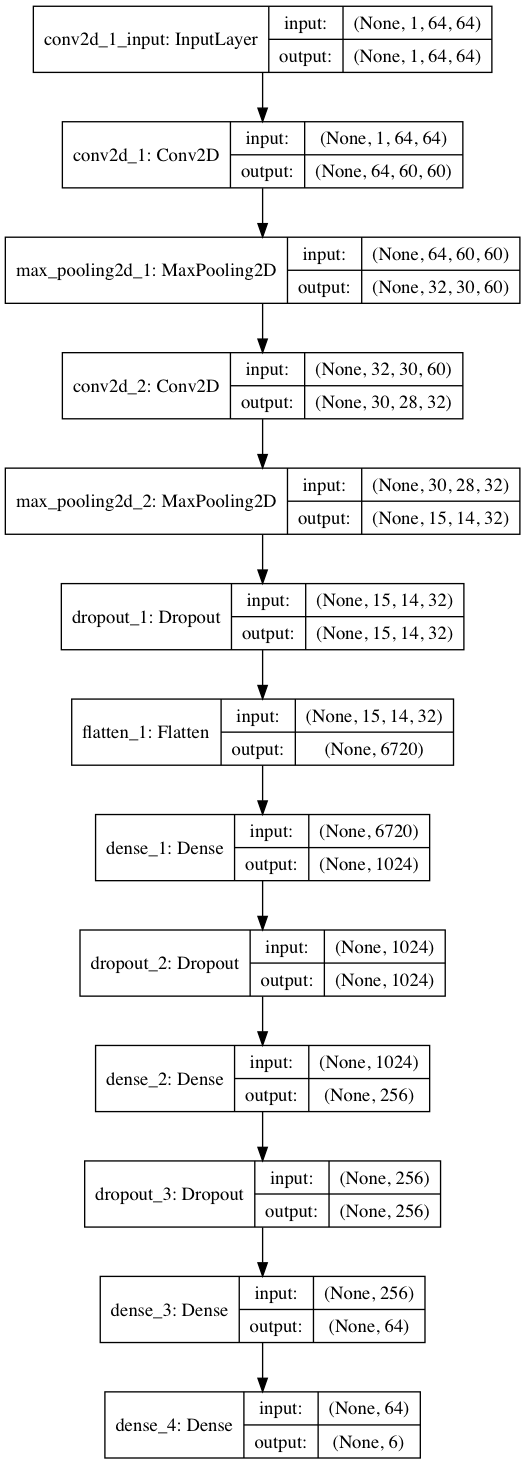
\includegraphics[scale=0.35]{pierwszy_plot}
\caption{Pierwszy model sieci}
\label{fig:first_model}
\end{figure}
Ta oraz wszystkie kolejne sieci korzystają z ReLU jako funkcji aktywacji,
co pozwoliło na zmniejszenie ilości rożnic między modelami.\\
Na końcu każdej z sieci zastosowana jest funkcja softmax, która oblicza prawdopodobieństwo
wyrzucenia danej ilości oczek na kostce.\\\\
Rezultaty osiągnięte przez ten model były zdumiewające. Po pierwszej epoce
sieć uzyskała 61,98\% skuteczności ostatecznie osiągając wynik 99,88\% po 25 epokach.\\
Po analizie wyniku okazało się, że wykorzystanie wielu bardzo podobnych obrazów o identycznym
układzie barw, spowodowało występowanie niemal identycznych z treningowymi, zdjęć testowych.
Przy bardziej zróżnicowanych zdjęciach, wynik okazałby się zdecydowanie gorszy.
Występuje tu zjawisko przetrenowania, które pomimo bardzo dobrych wyników na zbiorze testowym,
w praktyce osiągałoby niezadowalające rezultaty. Poniżej znajdują się wykresy (zob. rys. \ref{fig:first_plots})
dla sieć w kolejnych epokach:

\begin{figure}[h!]
\begin{center}
\begin{tabular}{cc}
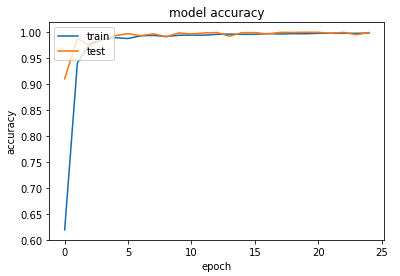
\includegraphics[width=0.49\linewidth]{pierwszy_acc.png} &
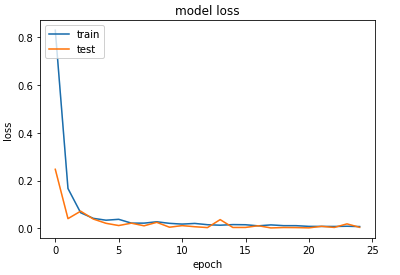
\includegraphics[width=0.49\linewidth]{pierwszy_loss.png} \\
 Skuteczność rozpoznawania kości & Wartość funkcji błędu\\
\end{tabular}
\captionof{figure}{Wykresy dla pierwszego modelu}
\label{fig:first_plots}
\end{center}
\end{figure}

\paragraph{Model ze zróżnicowanymi zdjęciami} \mbox{}\\
Po stworzeniu modelu, który wykazał, że zadanie stworzenia dobrze działającej sieci dla
tego problemu jest wykonalne, zabrano się do kolejnego etapu prac. W tym celu
wykorzystano opisany w poprzednim rozdziale zbiór obrazów kwadratowych złożony ze 100800 zdjęć
podzielonych na 80640 i 20160 w części treningowej i testowej.\\
W modelu wykorzystano architekturę nieznacznie zmienioną w stosunku do pierwszego modelu.
Poniżej znajduje się opisywany model (zob. rys. \ref{fig:adam}): \newpage

\begin{figure}[h!]
\centering
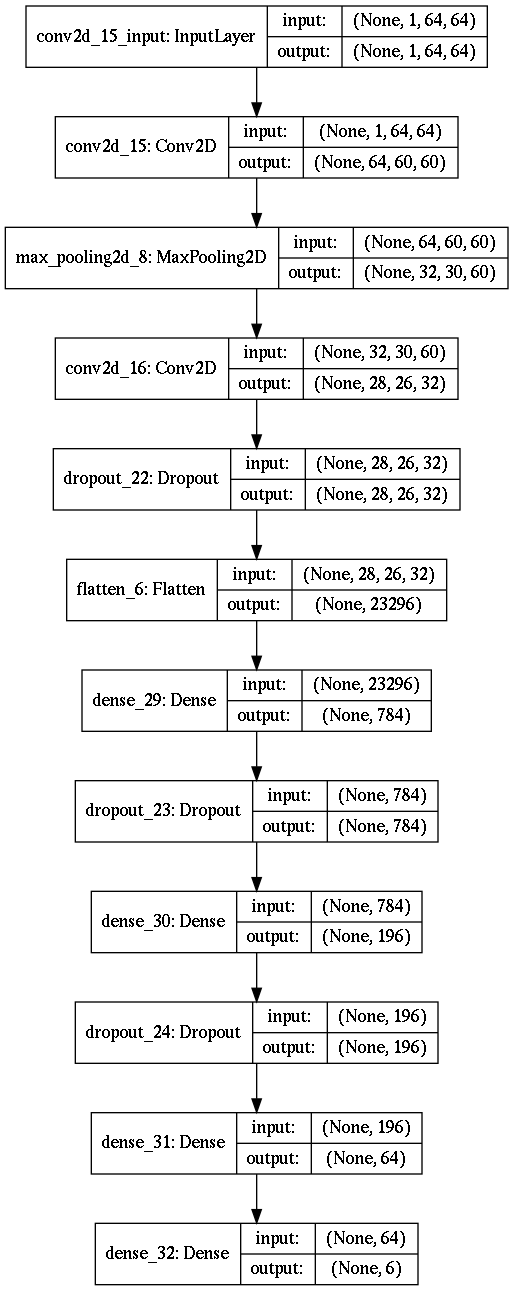
\includegraphics[scale=0.35]{modeladam_plot}
\caption{Model bazujący na optymalizatorze Adam}
\label{fig:adam}
\end{figure}
Tak jak poprzednio sieć uczona była przez 25 epok.
Po pierwszych 25 epokach uzyskano dokładność 55,64\% co potwierdziło przypuszczenie
z poprzedniej sieci o przetrenowaniu i konieczności zróżnicowania danych.
Poniżej znajdują się wykresy (zob. rys. \ref{fig:adam_plots}) uczenia się modelu:
\newpage
\begin{figure}[h!]
\begin{center}
\begin{tabular}{cc}
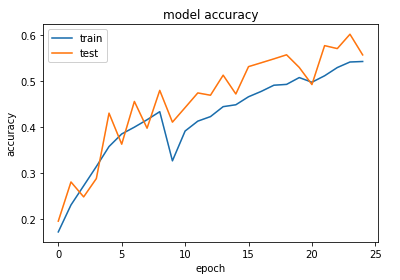
\includegraphics[width=0.49\linewidth]{adam_acc} &
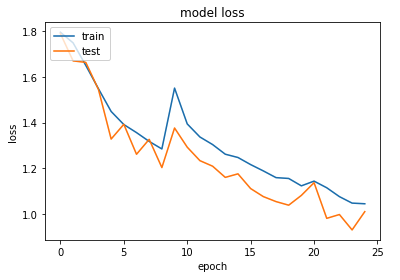
\includegraphics[width=0.49\linewidth]{adam_loss} \\
 Skuteczność rozpoznawania kości & Wartość funkcji błędu\\
\end{tabular}
\captionof{figure}{Wykresy dla modelu z optymalizatorem Adam}
\label{fig:adam_plots}
\end{center}
\end{figure}

\paragraph{Model z wybranymi zdjęciami} \mbox{}\\
Kolejnym punktem sprawdzenia jak zróżnicowanie danych wpływa na wyniki sieci, było
wykorzystanie tylko niektórych zestawów danych z całego zbioru 100800 kwadratowych obrazów.
Zestawy były dobrane tak, by kontrast między tłem a kością był wyraźny. Architektura sieci
była identyczna z powyższym przykładem. 25 epok wystarczyło do uzyskania dokładności
na poziomie 89,23\% co jest rezultatem zdecydowanie lepszym niż uzyskane wcześniej 55,64\%.\\
Przebieg uczenia sieci widoczny jest poniżej (zob. rys. \ref{fig:chosen_plots}): \newpage

\begin{figure}[h!]
\begin{center}
\begin{tabular}{cc}
\includegraphics[width=0.49\linewidth]{adam_chosen_acc} &
\includegraphics[width=0.49\linewidth]{adam_chosen_loss} \\
 Skuteczność rozpoznawania kości & Wartość funkcji błędu\\
\end{tabular}
\captionof{figure}{Wykresy dla modelu korzystającego z wybranych zestawów kolorystycznych}
\label{fig:chosen_plots}
\end{center}
\end{figure}

\section{Analiza różnych optymalizatorów}
Następnym krokiem analizy sieci neuronowych było przetestowaniu kilku z dostępnych
w bibliotece Keras optymalizatorów dla identycznych sieci. Zbiorem danych był
opisany w poprzednim rozdziale zbiór złożony z 100800 kwadratowych obrazów.
W tym celu postanowiono użyć optymalizatorów RMSprop oraz SGD.\\
Oba modele z optymalizatorami RMSprop oraz SGD zostały, podobnie jak wcześniej opisany model
z Adam, poddane uczeniu przez 25 epok różnorodnych zbiorów obrazów. Wynik RMSprop
był zdecydowanie wyróżniający się i wyniósł 84,34\% skuteczności. Najgorszy rezultat w zestawieniu
uzyskał model korzystający z SGD, zdobywając jedynie 36,92\% poprawności. Pośrednim okazał
się Adam, który jak opisane wyżej, uzyskał 55,64\% po sesji uczenia przez 25 epok.\\
Wyniki te dowiodły, że optymalizator jest kluczowym parametrem \textit{(ang. hyperparameter)}
dla odpowiednio skutecznego uczenia. Uzyskany wynik dla RMSprop jest sporym zaskoczeniem,
ponieważ w licznych tekstach naukowych to Adam uznawany jest za jeden z najlepszych
optymalizatorów, ciesząc się ogromną popularnością. Również z tego powodu, pomimo
gorszego niż RMSprop wyniku, Adam będzie wykorzystywany w następnych modelach.
Poniżej znajdują się wyniki dla każdego z analizowanych optymalizatorów
(zob. rys. \ref{fig:comparison_adam}, \ref{fig:comparison_rmsprop}, \ref{fig:comparison_sgd}):

\begin{figure}[h!]
\begin{center}
\begin{tabular}{cc}
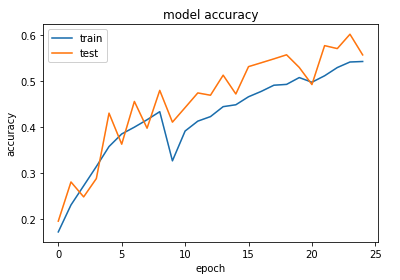
\includegraphics[width=0.49\linewidth]{adam_acc} &
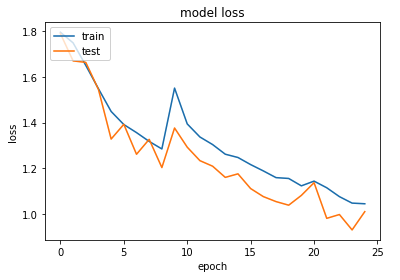
\includegraphics[width=0.49\linewidth]{adam_loss} \\
 Skuteczność rozpoznawania kości & Wartość funkcji błędu\\
\end{tabular}
\captionof{figure}{Wykresy dla modelu korzystającego z optymalizatora Adam}
\label{fig:comparison_adam}
\end{center}
\end{figure}

\begin{figure}[h!]
\begin{center}
\begin{tabular}{cc}
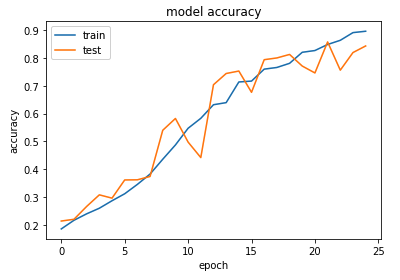
\includegraphics[width=0.49\linewidth]{rmsprop_acc} &
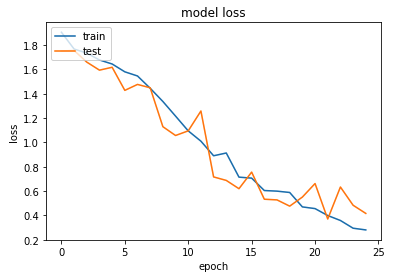
\includegraphics[width=0.49\linewidth]{rmsprop_loss} \\
 Skuteczność rozpoznawania kości & Wartość funkcji błędu\\
\end{tabular}
\captionof{figure}{Wykresy dla modelu korzystającego z optymalizatora RMSprop}
\label{fig:comparison_rmsprop}
\end{center}
\end{figure}

\begin{figure}[h!]
\begin{center}
\begin{tabular}{cc}
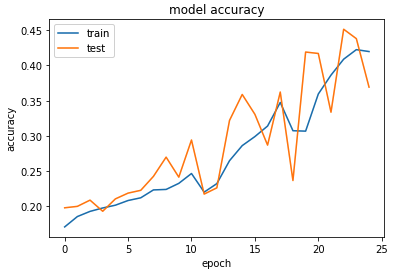
\includegraphics[width=0.49\linewidth]{sgd_acc} &
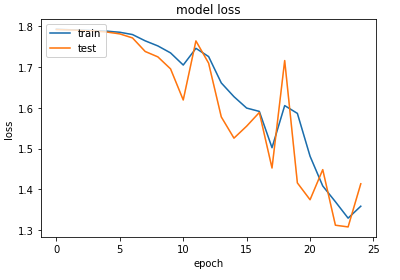
\includegraphics[width=0.49\linewidth]{sgd_loss} \\
 Skuteczność rozpoznawania kości & Wartość funkcji błędu\\
\end{tabular}
\captionof{figure}{Wykresy dla modelu korzystającego z optymalizatora SGD}
\label{fig:comparison_sgd}
\end{center}
\end{figure}
\newpage

\section{Wykorzystanie sieci AlexNet}
Sieć o nazwie AlexNet \cite{AlexNetNVIDIA, AlexNetpresentation} została
zaprezentowana przez Alexa Krizhevskyego, Geoffreya Hintona oraz Ilya Sutskevera w 2012 roku.
Jej ideą jest zastosowanie większej ilości warstw konwolucyjnych, gdzie początkowe dwie warstwy
mają filtry rozmiarów odpowiednio 11x11 oraz 5x5. Następnie umieszczone są trzy warstwy
konwolucyjne z filtrami 3x3, które w przeciwieństwie do pierwszych
dwóch warstw nie są rozdzielone warstwami z maxpoolingiem. AlexNet zdeklasowała rywali
w konkursie ILSVRC 2012 na rozpoznawanie obrazów. Dzięki świetnym
wynikom, zdecydowano się na realizację modelu przypominającego jej budowę.
Zastosowano model bazujący na idei AlexNet, z uproszczoną architekturą, która przedstawiona jest poniżej (zob. rys. \ref{fig:alexnet}):
\newpage
\begin{figure}[h!]
\centering
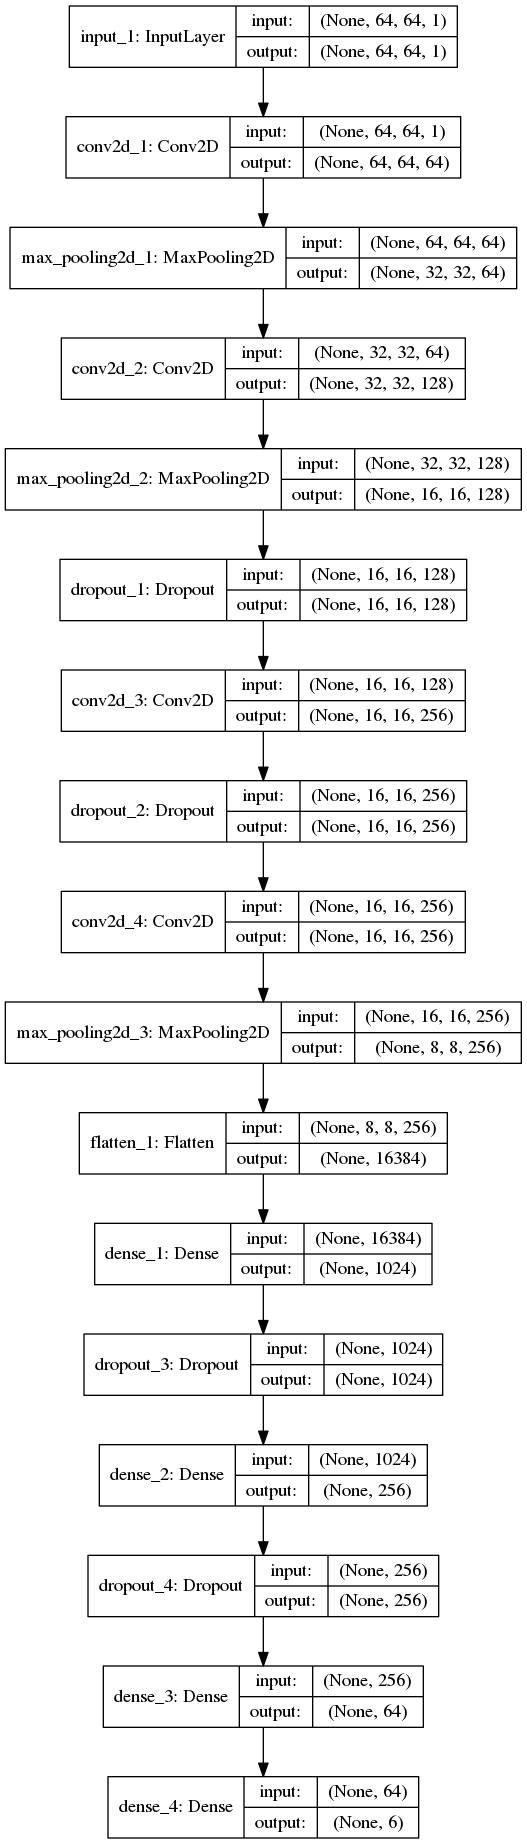
\includegraphics[scale=0.35]{dice_AlexNet_plot}
\caption{Model bazujący na Alexnet}
\label{fig:alexnet}
\end{figure}
Na zbiorze 100800 kwadratowych obrazów, po 25 epokach osiągnięto poprawność wynoszącą aż 98.88\%.
Na wykresach uczenia (zob. rys. \ref{fig:alexnet_plot}) można zaobserwować, że przez pierwsze 10 epok precyzja przewidywań
i wartość funkcji kosztu sieci praktycznie się nie zmieniały. Obserwacja sugeruje, że sieci
głębsze mogą potrzebować większej ilości epok do rozpoczęcia procesu prawidłowego rozpoznawania obrazów.\\
\begin{figure}[h!]
\begin{center}
\begin{tabular}{cc}
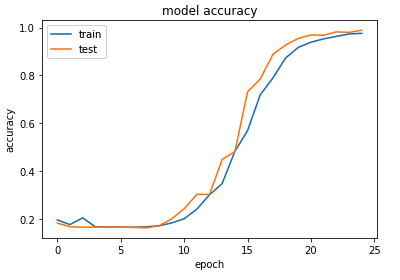
\includegraphics[width=0.49\linewidth]{alexnet_acc} &
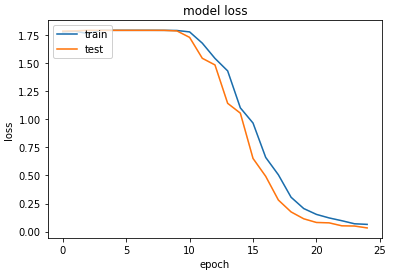
\includegraphics[width=0.49\linewidth]{alexnet_loss} \\
 Skuteczność rozpoznawania kości & Wartość funkcji błędu\\
\end{tabular}
\captionof{figure}{Wykresy dla sieci opartej o AlexNet}
\label{fig:alexnet_plot}
\end{center}
\end{figure}\\

\section{Porównanie dla obrazów kolorowych i czarno-białych}
Obraz w skali szarości posiada jedynie jeden kanał odpowiadający jasności. Obrazy kolorowe RGB
posiadają trzy kanały informujące o nasyceniu odpowiednio czerwonego, zielonego i niebieskiego koloru.
Wzrost ilości informacji wiąże się z większym obciążeniem pamięci i większą ilością parametrów.
W celu weryfikacji różnicy między uczeniem obu rodzajów obrazów podjęto próbę porównania wyników
uczenia dla dwóch jednakowych sieci. Pierwsza z sieci korzystała z kolorowej wersji zbioru
obrazów kwadratowych, dla których zastosowano kąt obrotu 30\textsuperscript{o}, uzyskując
50400 obrazów. Sieć korzystająca z czarno-białych obrazów miała te same zdjęcia z jednym
zamiast trzech kanałów informujących o kolorze. Do tego eksperymentu
wykorzystano narzędzie generatora dostępne w Keras, które przekazuje obrazy do sieci
bez konieczności wcześniejszego ładowania całego zbioru do pamięci. Architektura obu
sieci była uproszczona, by zniwelować długi czas uczenia. Wykresy (zob. rys. \ref{fig:comp_color}) przedstawiają
proces uczenia na obrazach kolorowych, a wykresy (zob. rys. \ref{fig:comp_gray}) na obrazach w odcieniach skali szarości:\\
\begin{figure}[h!]
\begin{center}
\begin{tabular}{cc}
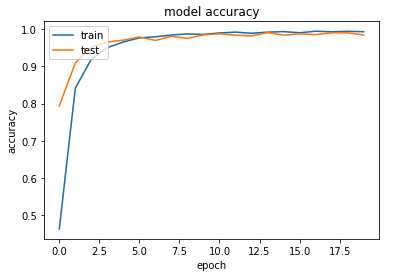
\includegraphics[width=0.49\linewidth]{comp_color_acc} &
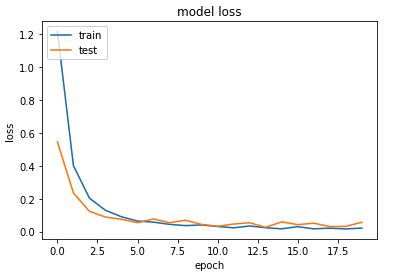
\includegraphics[width=0.49\linewidth]{comp_color_loss} \\
 Skuteczność rozpoznawania kości & Wartość funkcji błędu\\
\end{tabular}
\captionof{figure}{Wykresy dla sieci z obrazami kolorowymi}
\label{fig:comp_color}
\end{center}
\end{figure}
\begin{figure}[h!]
\begin{center}
\begin{tabular}{cc}
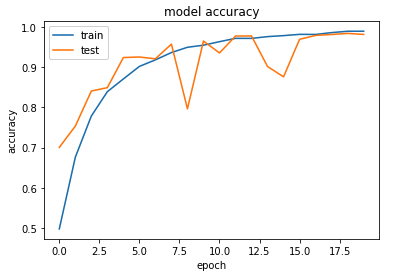
\includegraphics[width=0.49\linewidth]{comp_gray_acc} &
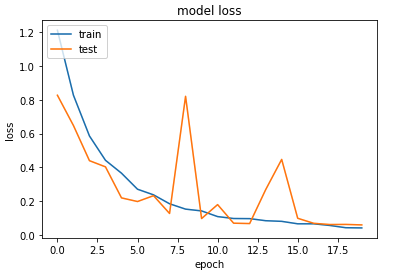
\includegraphics[width=0.49\linewidth]{comp_gray_loss} \\
 Skuteczność rozpoznawania kości & Wartość funkcji błędu\\
\end{tabular}
\captionof{figure}{Wykresy dla sieci z obrazami w skali szarości}
\label{fig:comp_gray}
\end{center}
\end{figure}\newpage
Jak można zauważyć, oba modele po 20 epokach wykazały się bardzo zbliżonymi wynikami 98,47\% oraz 98,12\%
na korzyść sieci z kolorowymi obrazami. Model z lepszym wynikiem nauczył się bardzo szybko
do poziomu 95\%, osiągając go już po 4 epoce, gdzie drugi osiągnął ten wynik po 10 epokach.
Obserwacja ta może sugerować, że większa różnica w wartościach dla kolorowych obrazów
może przyśpieszać uczenie, ale wymaga większej ilości pamięci i spowalnia każdą epokę o 15\%.

\section{Próby wykorzystania prostokątnych obrazów}
Dotychczasowe modele korzystały ze zbiorów o obrazach w kształcie kwadratów z kośćmi
umieszczonymi w ich środkowej części. Drugi rodzaj przygotowanych zbiorów danych zwiększał
trudność zadania, dzięki zastosowaniu obrazów prostokątnych z proporcjonalnie mniejszym
rozmiarem kości w stosunku do pierwszego rodzaju obrazów.\\
Po uzyskaniu wielu bardzo dobrych wyników powyżej 90\% na obrazach o rozmiarach 64x64
przystąpiono do prób ze znacznie zwiększonymi obrazami prostokątnymi.\\
Pierwszą próbą było wykorzystanie obrazów 320x240 zarówno w wersjach kolorowych, jak i w skali szarości.
Jeden z modeli bazował na architekturze AlexNet, drugi bezpośrednio
ją kopiował, ale pomimo świetnego wyniku na mniejszych obrazach, w obu przypadkach
uczenie zakończyło się całkowitą klęską. Przez wszystkie 25 epok skuteczność rozpoznawania
nie poprawiła się w żadnym stopniu. Warto wspomnieć, że czas potrzebny na
jedną epokę był około 15-krotnie większy niż w przypadku obrazów 64x64.\\
Ostania próba z obrazami w tym rozmiarze zakładała użycie uproszczonej architektury,
podobnie jak przy porównaniu uczenia obrazów RGB i w skali szarości. Finalnie, tak jak
wcześniej, pomimo 20 epok sieć nie wykazała żadnego postępu w rozpoznawaniu kości.\\\\
Niepowodzenia spowodowały konieczność zmniejszenia ilości danych do przetworzenia przez ograniczenie rozmiarów obrazów.
Kluczowa przy tym była chęć uniknięcia problemów z brakiem ostrości
oczek na kostce co mogłoby uniemożliwić skuteczną naukę. Zdecydowano się na dwukrotne
zmniejszenie rozmiarów obrazów, licząc, że pozwoli to na zaobserwowanie, chociaż niewielkich
postępów.\\
Sieć bazująca na zdjęciach 160x120 była pierwszą próbą, gdzie zamiast jak dotychczas
kwadratowych, użyto prostokątnych filtrów konwolucyjnych. Proces uczenia po 20 epokach
niestety również zakończył się niepowodzeniem. Wykresy (zob. rys. \ref{fig:not_learned}) uczenia się przedstawione sa poniżej: \newpage

\begin{figure}[h!]
\begin{center}
\begin{tabular}{cc}
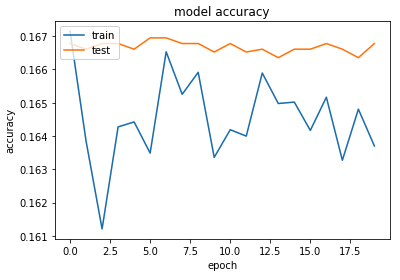
\includegraphics[width=0.49\linewidth]{not_learned_acc} &
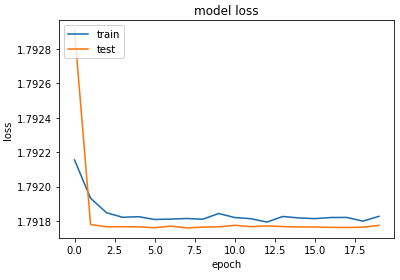
\includegraphics[width=0.49\linewidth]{not_learned_loss} \\
 Skuteczność rozpoznawania kości & Wartość funkcji błędu\\
\end{tabular}
\captionof{figure}{Wykresy dla nienauczonej sieci z obrazami 160x120}
\label{fig:not_learned}
\end{center}
\end{figure}

\paragraph{Wytrenowany prostokątny model} \mbox{}\\
Powyższe porażki oraz wcześniejsze sukcesy na kwadratowych obrazach sugerowały, że
obrazy mogą mieć za duży rozmiar. To przypuszczenie rozpoczęło dobieranie
odpowiedniej rozdzielczości zdjęć tak by rozmiar był mały, a jednocześnie nie powodował
zanikania informacji o oczkach na kostce. Najlepszym wyborem okazały się zdjęcia w rozmiarze 106x79,
zachowujące proporcje identyczne z obrazami 160x120, ale posiadające o 50\% mniejszą liczbę parametrów.
Poniżej przedstawiony jest model tej sieci (zob. rys. \ref{fig:simple_106x79}):
\newpage
\begin{figure}[h!]
\centering
\includegraphics[scale=0.35]{simple_NN_106x79_plot.png}
\caption{Model bazujący na Alexnet}
\label{fig:simple_106x79}
\end{figure}
Pierwsza próba przeprowadzona przez 20 epok z filtrami konwolucjnymi o prostokątnych
kształtach wreszcie zakończyła się sukcesem. Sieć osiągnęła wynik 68,03\% co nie
było świetnym rezultatem, ale sugerowało, że dalsza nauka jest możliwa. Wykres (zob. rys. \ref{fig:rect_learned}) uczenia znajduje się poniżej.\\

\begin{figure}[h!]
\begin{center}
\begin{tabular}{cc}
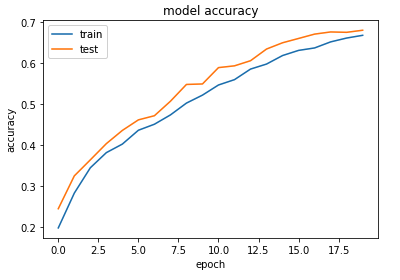
\includegraphics[width=0.49\linewidth]{rect_acc} &
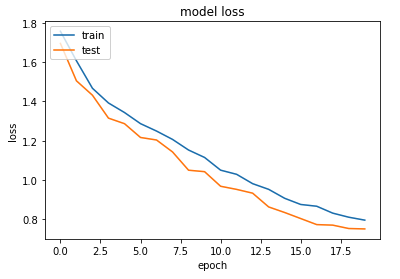
\includegraphics[width=0.49\linewidth]{rect_loss} \\
 Skuteczność rozpoznawania kości & Wartość funkcji błędu\\
\end{tabular}
\captionof{figure}{Wykresy dla nauczonej sieci z obrazami 106x79}
\label{fig:rect_learned}
\end{center}
\end{figure}

\section{Najskuteczniejszy model z prostokątnymi obrazami}
Wyżej przedstawiony wykres uczenia kształtem przypominał funkcję logarytmiczną, co wskazywało na możliwość 
dalszej nauki sieci z obrazami 106x79 pikseli. Nauka była kontynuowana do kolejno 40, 60, 80 i 100 epok.\\
Podejście to okazało się bardzo skuteczne, ponieważ po każdych 20 epokach
sieć odnosiła coraz lepsze rezultaty, które prezentowały się następująco:\\
\begin{itemize}
\item  20 epok: 68,03\%\\
\item  40 epok: 78,21\%\\
\item  60 epok: 81,59\%\\
\item  80 epok: 82,39\%\\
\item  100 epok: 84,67\%\\
\end{itemize}
Wyniki uświadamiają, że prawdopodobnie nawet nieudane próby z większymi zdjęciami
mogłyby się powieść, konieczne byłoby jedynie zwiększenie ilości epok. Wiąże się to
z ogromnym nakładem czasu, ponieważ prawdopodobnie sensowne rezultaty można by osiągnąć
dopiero po 100 epokach. Wykres (zob. rys. \ref{fig:sideway_fig}) dokładności sieci znajduje się na następnej stronie.

\begin{sidewaysfigure}
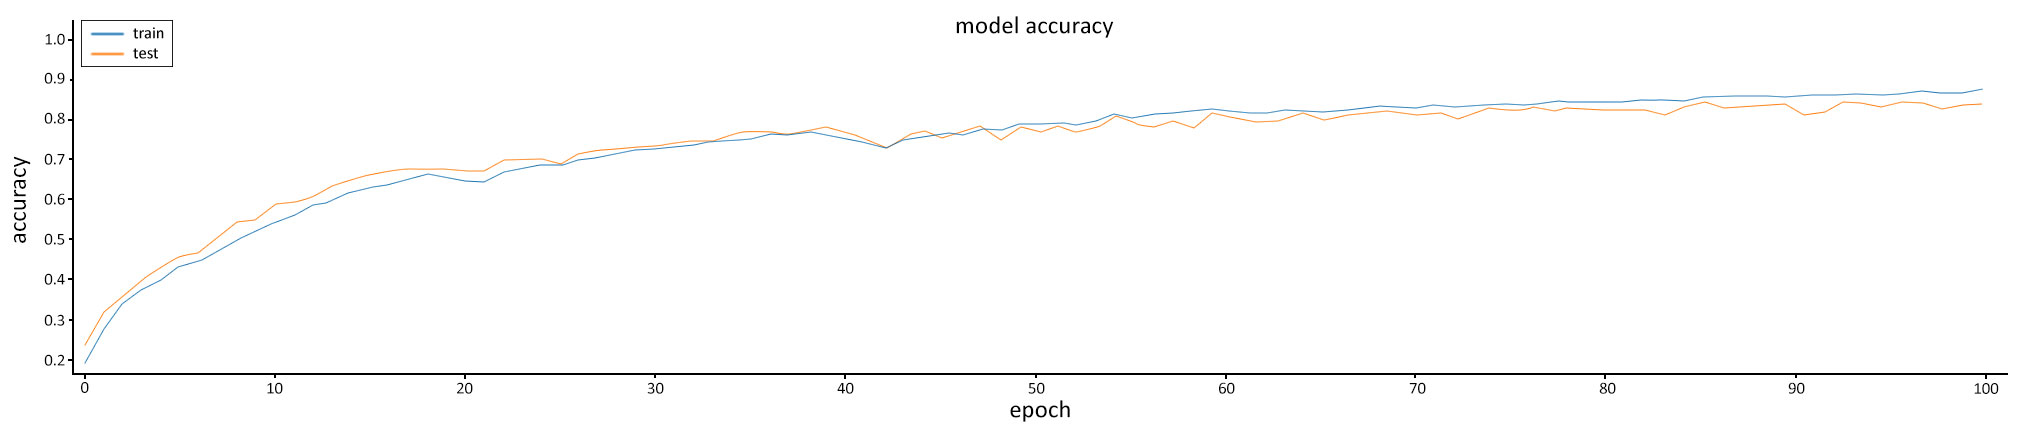
\includegraphics[scale=0.36]{wykres_100}
\caption{Wykres uczenia przez 100 epok}
\label{fig:sideway_fig}
\end{sidewaysfigure}

\section{Doskonalenie modelu z prostokątnymi obrazami}
Po sukcesie sieci z obrazami prostokątnymi podjęto decyzję o jej ulepszeniu.
Zaczęto od próby zmniejszenia ilości parametrów przez zamianę większych filtrów konwolucyjnych,
większą ilością mniejszych. Zabieg ten znacząco zmniejszał ilość parametrów sieci potrzebną do nauczenia \cite{substBigConv}.
Po zaaplikowaniu ulepszeń i nauce sieci okazało się, że model nie poprawił się w żadnym
stopniu. Prawdopodobnym powodem była zmiana architektury sieci wraz z powtórnym
zastosowaniem kwadratowych filtrów.\\
Drugim pomysłem na ulepszenie sieci było zastosowanie zastępowania większych filtrów
kilkoma mniejszymi. Dodatkowo w celu uniknięcia problemów z zanikającym neuronem zmieniono z ReLU na LeakyReLU.
Ulepszenie jednak podobnie jak wcześniejsze nie sprawdziło się w ogóle i nie umożliwiło poprawy dokładności sieci.
